\section{Arquitetura}

\subsection{Linguagem}

O aplicativo Guimifiu está sendo desenvolvendo utilizando o framework Ionic 2, que por sua vez utiliza Typescript como linguagem de programação. O Typescript é uma linguagem que facilita o desenvolvimento em JavaScript em larga escala. É uma linguagem fortemente tipada, e que facilita a aplicação de orientação a objetos em aplicações JavaScript. O Typescript é compilado e transformado em JavaScript \cite{typescript}.
Em conjunto com o desenvolvimento do aplicativo, está sendo desenvolvido uma API RESTful utilizando a linguagem de programação Ruby com o framework Ruby on Rails. A representação dos dados da API são em JSON.


\subsection{Representação da Arquitetura}

A forma como está sendo utilizado o framework Ionic pode ser representado com diagrama de pacotes representado na figura \ref{img:pacotes}:

\begin{figure}[H]
    \centering
    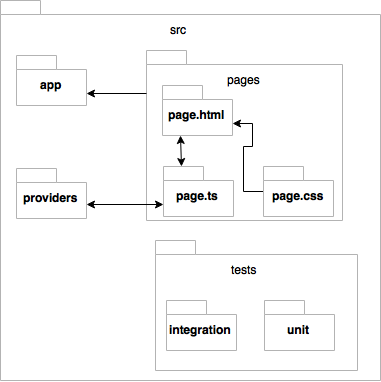
\includegraphics[scale=0.5]{figuras/ionic_arch.png}
    \caption[Diagrama de pacotes do aplicativo]{Diagrama de pacotes.}
    \label{img:pacotes}
\end{figure}

A arquitetura da API é baseada na arquitetura MVC (Model View Controller) e está definida como ilustra a figura \ref{img:arquitetura}:

\begin{figure}[H]
    \centering
    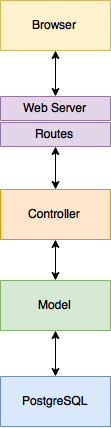
\includegraphics[scale=0.5]{figuras/api_arch.png}
    \caption[Arquitetura da API]{Arquitetura da API.}
    \label{img:arquitetura}
\end{figure}


\subsection{Modelo de Dados}

O modelo da aplicação é representado pela figura \ref{img:modelo_de_dados}:

\begin{figure}[H]
    \centering
    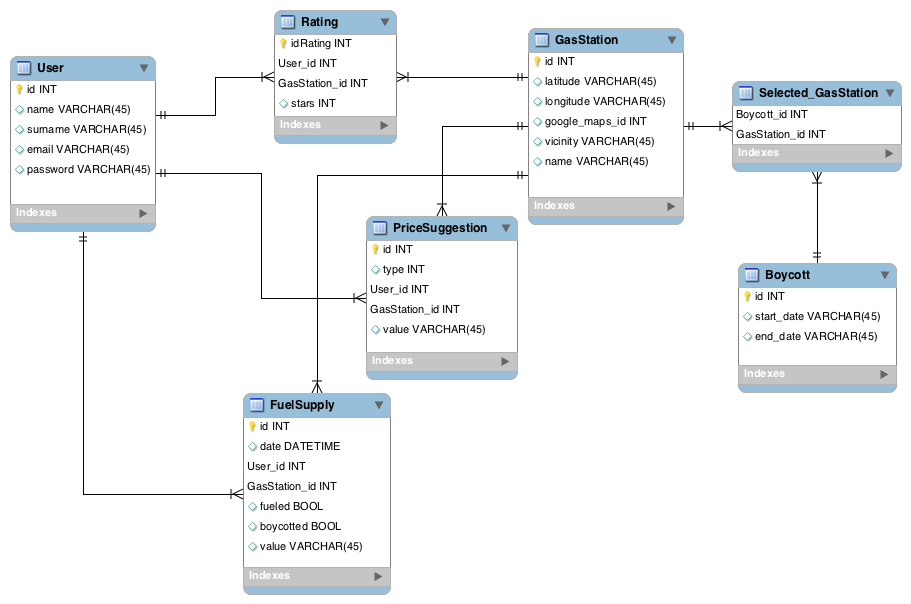
\includegraphics[scale=0.5]{figuras/db_model.png}
    \caption[Modelo de dados]{Modelo de dados}
    \label{img:modelo_de_dados}
\end{figure}
